\documentclass[a4paper,12pt]{article}
\usepackage[margin=18mm]{geometry}
\usepackage{tikz}
\usepackage[T1]{fontenc}
\usepackage[utf8]{inputenc}
\usepackage{xcolor}
\pagestyle{empty}
\begin{document}
\section*{Spaltentreue Umbauansicht}
\noindent Gleichung: \texttt{a*x+3=5} \hfill Zielvariable: \texttt{x}

\vspace{8mm}
\begin{center}
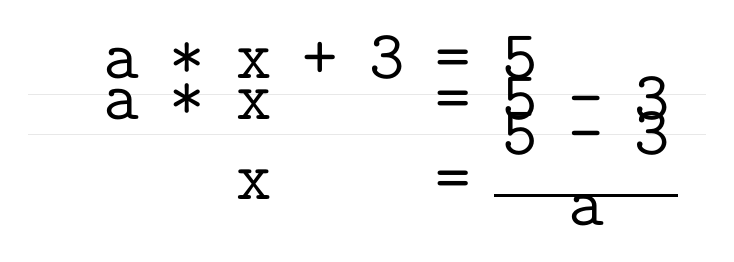
\begin{tikzpicture}[x=2.4em, y=-1em]
\draw[gray!18] (-1.4,1.67) -- (8.8,1.67);
\draw[gray!18] (-1.4,3.13) -- (8.8,3.13);
\node[anchor=base, font={\ttfamily\fontsize{24}{24}\selectfont}] at (0,1.12) {a};
\node[anchor=base, font={\ttfamily\fontsize{24}{24}\selectfont}] at (1,1.12) {*};
\node[anchor=base, font={\ttfamily\fontsize{24}{24}\selectfont}] at (2,1.12) {x};
\node[anchor=base, font={\ttfamily\fontsize{24}{24}\selectfont}] at (3,1.12) {+};
\node[anchor=base, font={\ttfamily\fontsize{24}{24}\selectfont}] at (4,1.12) {3};
\node[anchor=base, font={\ttfamily\fontsize{24}{24}\selectfont}] at (5,1.12) {=};
\node[anchor=base, font={\ttfamily\fontsize{24}{24}\selectfont}] at (6,1.12) {5};
\node[anchor=base, font={\ttfamily\fontsize{24}{24}\selectfont}] at (0,2.58) {a};
\node[anchor=base, font={\ttfamily\fontsize{24}{24}\selectfont}] at (1,2.58) {*};
\node[anchor=base, font={\ttfamily\fontsize{24}{24}\selectfont}] at (2,2.58) {x};
\node[anchor=base, font={\ttfamily\fontsize{24}{24}\selectfont}] at (5,2.58) {=};
\node[anchor=base, font={\ttfamily\fontsize{24}{24}\selectfont}] at (6,2.58) {5};
\node[anchor=base, font={\ttfamily\fontsize{24}{24}\selectfont}] at (7,2.58) {-};
\node[anchor=base, font={\ttfamily\fontsize{24}{24}\selectfont}] at (8,2.58) {3};
\node[anchor=base, font={\ttfamily\fontsize{24}{24}\selectfont}] at (6,3.85) {5};
\node[anchor=base, font={\ttfamily\fontsize{24}{24}\selectfont}] at (7,3.85) {-};
\node[anchor=base, font={\ttfamily\fontsize{24}{24}\selectfont}] at (8,3.85) {3};
\node[anchor=base, font={\ttfamily\fontsize{24}{24}\selectfont}] at (2,5.49) {x};
\node[anchor=base, font={\ttfamily\fontsize{24}{24}\selectfont}] at (5,5.49) {=};
\draw[line width=0.1em, black] (5.62,5.34) -- (8.38,5.34);
\node[anchor=base, font={\ttfamily\fontsize{24}{24}\selectfont}] at (7,6.4) {a};
\end{tikzpicture}
\end{center}

\newpage
\section*{Projektionsraster}
\noindent Dieselben Daten mit Spaltenraster und Schrittmarkern.

\vspace{6mm}
\begin{center}
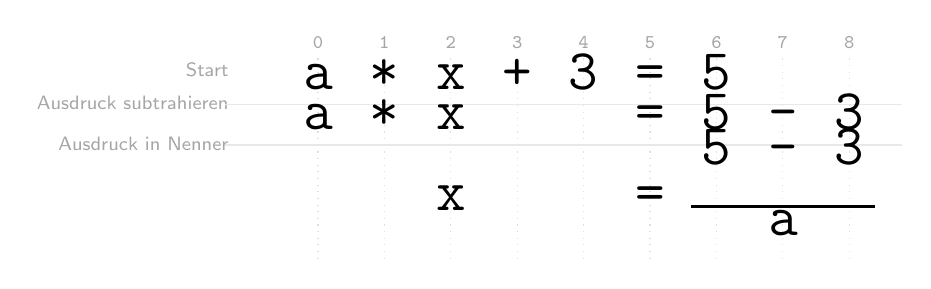
\begin{tikzpicture}[x=2.4em, y=-1em]
\draw[gray!25, dotted] (0,0) -- (0,7.3);
\node[anchor=base, font={\ttfamily\scriptsize}, text=gray!70] at (0,-0.35) {0};
\draw[gray!25, dotted] (1,0) -- (1,7.3);
\node[anchor=base, font={\ttfamily\scriptsize}, text=gray!70] at (1,-0.35) {1};
\draw[gray!25, dotted] (2,0) -- (2,7.3);
\node[anchor=base, font={\ttfamily\scriptsize}, text=gray!70] at (2,-0.35) {2};
\draw[gray!25, dotted] (3,0) -- (3,7.3);
\node[anchor=base, font={\ttfamily\scriptsize}, text=gray!70] at (3,-0.35) {3};
\draw[gray!25, dotted] (4,0) -- (4,7.3);
\node[anchor=base, font={\ttfamily\scriptsize}, text=gray!70] at (4,-0.35) {4};
\draw[gray!25, dotted] (5,0) -- (5,7.3);
\node[anchor=base, font={\ttfamily\scriptsize}, text=gray!70] at (5,-0.35) {5};
\draw[gray!25, dotted] (6,0) -- (6,7.3);
\node[anchor=base, font={\ttfamily\scriptsize}, text=gray!70] at (6,-0.35) {6};
\draw[gray!25, dotted] (7,0) -- (7,7.3);
\node[anchor=base, font={\ttfamily\scriptsize}, text=gray!70] at (7,-0.35) {7};
\draw[gray!25, dotted] (8,0) -- (8,7.3);
\node[anchor=base, font={\ttfamily\scriptsize}, text=gray!70] at (8,-0.35) {8};
\node[anchor=east, font={\sffamily\scriptsize}, text=gray!70] at (-1.2,0.4) {Start};
\node[anchor=east, font={\sffamily\scriptsize}, text=gray!70] at (-1.2,1.62) {Ausdruck subtrahieren};
\node[anchor=east, font={\sffamily\scriptsize}, text=gray!70] at (-1.2,3.08) {Ausdruck in Nenner};
\draw[gray!18] (-1.4,1.67) -- (8.8,1.67);
\draw[gray!18] (-1.4,3.13) -- (8.8,3.13);
\node[anchor=base, font={\ttfamily\fontsize{22}{22}\selectfont}] at (0,1.12) {a};
\node[anchor=base, font={\ttfamily\fontsize{22}{22}\selectfont}] at (1,1.12) {*};
\node[anchor=base, font={\ttfamily\fontsize{22}{22}\selectfont}] at (2,1.12) {x};
\node[anchor=base, font={\ttfamily\fontsize{22}{22}\selectfont}] at (3,1.12) {+};
\node[anchor=base, font={\ttfamily\fontsize{22}{22}\selectfont}] at (4,1.12) {3};
\node[anchor=base, font={\ttfamily\fontsize{22}{22}\selectfont}] at (5,1.12) {=};
\node[anchor=base, font={\ttfamily\fontsize{22}{22}\selectfont}] at (6,1.12) {5};
\node[anchor=base, font={\ttfamily\fontsize{22}{22}\selectfont}] at (0,2.58) {a};
\node[anchor=base, font={\ttfamily\fontsize{22}{22}\selectfont}] at (1,2.58) {*};
\node[anchor=base, font={\ttfamily\fontsize{22}{22}\selectfont}] at (2,2.58) {x};
\node[anchor=base, font={\ttfamily\fontsize{22}{22}\selectfont}] at (5,2.58) {=};
\node[anchor=base, font={\ttfamily\fontsize{22}{22}\selectfont}] at (6,2.58) {5};
\node[anchor=base, font={\ttfamily\fontsize{22}{22}\selectfont}] at (7,2.58) {-};
\node[anchor=base, font={\ttfamily\fontsize{22}{22}\selectfont}] at (8,2.58) {3};
\node[anchor=base, font={\ttfamily\fontsize{22}{22}\selectfont}] at (6,3.85) {5};
\node[anchor=base, font={\ttfamily\fontsize{22}{22}\selectfont}] at (7,3.85) {-};
\node[anchor=base, font={\ttfamily\fontsize{22}{22}\selectfont}] at (8,3.85) {3};
\node[anchor=base, font={\ttfamily\fontsize{22}{22}\selectfont}] at (2,5.49) {x};
\node[anchor=base, font={\ttfamily\fontsize{22}{22}\selectfont}] at (5,5.49) {=};
\draw[line width=0.1em, black] (5.62,5.34) -- (8.38,5.34);
\node[anchor=base, font={\ttfamily\fontsize{22}{22}\selectfont}] at (7,6.4) {a};
\end{tikzpicture}
\end{center}
\end{document}
